\documentclass[]{article}
\usepackage{lmodern}
\usepackage{amssymb,amsmath}
\usepackage{ifxetex,ifluatex}
\usepackage{fixltx2e} % provides \textsubscript
\ifnum 0\ifxetex 1\fi\ifluatex 1\fi=0 % if pdftex
  \usepackage[T1]{fontenc}
  \usepackage[utf8]{inputenc}
\else % if luatex or xelatex
  \ifxetex
    \usepackage{mathspec}
  \else
    \usepackage{fontspec}
  \fi
  \defaultfontfeatures{Ligatures=TeX,Scale=MatchLowercase}
\fi
% use upquote if available, for straight quotes in verbatim environments
\IfFileExists{upquote.sty}{\usepackage{upquote}}{}
% use microtype if available
\IfFileExists{microtype.sty}{%
\usepackage{microtype}
\UseMicrotypeSet[protrusion]{basicmath} % disable protrusion for tt fonts
}{}
\usepackage[margin=1in]{geometry}
\usepackage{hyperref}
\hypersetup{unicode=true,
            pdftitle={Inférence bayésienne et méthodes MCMC},
            pdfauthor={Pierre Gloaguen},
            pdfborder={0 0 0},
            breaklinks=true}
\urlstyle{same}  % don't use monospace font for urls
\usepackage{color}
\usepackage{fancyvrb}
\newcommand{\VerbBar}{|}
\newcommand{\VERB}{\Verb[commandchars=\\\{\}]}
\DefineVerbatimEnvironment{Highlighting}{Verbatim}{commandchars=\\\{\}}
% Add ',fontsize=\small' for more characters per line
\usepackage{framed}
\definecolor{shadecolor}{RGB}{248,248,248}
\newenvironment{Shaded}{\begin{snugshade}}{\end{snugshade}}
\newcommand{\AlertTok}[1]{\textcolor[rgb]{0.94,0.16,0.16}{#1}}
\newcommand{\AnnotationTok}[1]{\textcolor[rgb]{0.56,0.35,0.01}{\textbf{\textit{#1}}}}
\newcommand{\AttributeTok}[1]{\textcolor[rgb]{0.77,0.63,0.00}{#1}}
\newcommand{\BaseNTok}[1]{\textcolor[rgb]{0.00,0.00,0.81}{#1}}
\newcommand{\BuiltInTok}[1]{#1}
\newcommand{\CharTok}[1]{\textcolor[rgb]{0.31,0.60,0.02}{#1}}
\newcommand{\CommentTok}[1]{\textcolor[rgb]{0.56,0.35,0.01}{\textit{#1}}}
\newcommand{\CommentVarTok}[1]{\textcolor[rgb]{0.56,0.35,0.01}{\textbf{\textit{#1}}}}
\newcommand{\ConstantTok}[1]{\textcolor[rgb]{0.00,0.00,0.00}{#1}}
\newcommand{\ControlFlowTok}[1]{\textcolor[rgb]{0.13,0.29,0.53}{\textbf{#1}}}
\newcommand{\DataTypeTok}[1]{\textcolor[rgb]{0.13,0.29,0.53}{#1}}
\newcommand{\DecValTok}[1]{\textcolor[rgb]{0.00,0.00,0.81}{#1}}
\newcommand{\DocumentationTok}[1]{\textcolor[rgb]{0.56,0.35,0.01}{\textbf{\textit{#1}}}}
\newcommand{\ErrorTok}[1]{\textcolor[rgb]{0.64,0.00,0.00}{\textbf{#1}}}
\newcommand{\ExtensionTok}[1]{#1}
\newcommand{\FloatTok}[1]{\textcolor[rgb]{0.00,0.00,0.81}{#1}}
\newcommand{\FunctionTok}[1]{\textcolor[rgb]{0.00,0.00,0.00}{#1}}
\newcommand{\ImportTok}[1]{#1}
\newcommand{\InformationTok}[1]{\textcolor[rgb]{0.56,0.35,0.01}{\textbf{\textit{#1}}}}
\newcommand{\KeywordTok}[1]{\textcolor[rgb]{0.13,0.29,0.53}{\textbf{#1}}}
\newcommand{\NormalTok}[1]{#1}
\newcommand{\OperatorTok}[1]{\textcolor[rgb]{0.81,0.36,0.00}{\textbf{#1}}}
\newcommand{\OtherTok}[1]{\textcolor[rgb]{0.56,0.35,0.01}{#1}}
\newcommand{\PreprocessorTok}[1]{\textcolor[rgb]{0.56,0.35,0.01}{\textit{#1}}}
\newcommand{\RegionMarkerTok}[1]{#1}
\newcommand{\SpecialCharTok}[1]{\textcolor[rgb]{0.00,0.00,0.00}{#1}}
\newcommand{\SpecialStringTok}[1]{\textcolor[rgb]{0.31,0.60,0.02}{#1}}
\newcommand{\StringTok}[1]{\textcolor[rgb]{0.31,0.60,0.02}{#1}}
\newcommand{\VariableTok}[1]{\textcolor[rgb]{0.00,0.00,0.00}{#1}}
\newcommand{\VerbatimStringTok}[1]{\textcolor[rgb]{0.31,0.60,0.02}{#1}}
\newcommand{\WarningTok}[1]{\textcolor[rgb]{0.56,0.35,0.01}{\textbf{\textit{#1}}}}
\usepackage{longtable,booktabs}
\usepackage{graphicx,grffile}
\makeatletter
\def\maxwidth{\ifdim\Gin@nat@width>\linewidth\linewidth\else\Gin@nat@width\fi}
\def\maxheight{\ifdim\Gin@nat@height>\textheight\textheight\else\Gin@nat@height\fi}
\makeatother
% Scale images if necessary, so that they will not overflow the page
% margins by default, and it is still possible to overwrite the defaults
% using explicit options in \includegraphics[width, height, ...]{}
\setkeys{Gin}{width=\maxwidth,height=\maxheight,keepaspectratio}
\IfFileExists{parskip.sty}{%
\usepackage{parskip}
}{% else
\setlength{\parindent}{0pt}
\setlength{\parskip}{6pt plus 2pt minus 1pt}
}
\setlength{\emergencystretch}{3em}  % prevent overfull lines
\providecommand{\tightlist}{%
  \setlength{\itemsep}{0pt}\setlength{\parskip}{0pt}}
\setcounter{secnumdepth}{5}
% Redefines (sub)paragraphs to behave more like sections
\ifx\paragraph\undefined\else
\let\oldparagraph\paragraph
\renewcommand{\paragraph}[1]{\oldparagraph{#1}\mbox{}}
\fi
\ifx\subparagraph\undefined\else
\let\oldsubparagraph\subparagraph
\renewcommand{\subparagraph}[1]{\oldsubparagraph{#1}\mbox{}}
\fi

%%% Use protect on footnotes to avoid problems with footnotes in titles
\let\rmarkdownfootnote\footnote%
\def\footnote{\protect\rmarkdownfootnote}

%%% Change title format to be more compact
\usepackage{titling}

% Create subtitle command for use in maketitle
\providecommand{\subtitle}[1]{
  \posttitle{
    \begin{center}\large#1\end{center}
    }
}

\setlength{\droptitle}{-2em}

  \title{Inférence bayésienne et méthodes MCMC}
    \pretitle{\vspace{\droptitle}\centering\huge}
  \posttitle{\par}
  \subtitle{Travaux dirigés}
  \author{Pierre Gloaguen}
    \preauthor{\centering\large\emph}
  \postauthor{\par}
    \date{}
    \predate{}\postdate{}
  
\usepackage{xcolor}
\usepackage{mdframed}
\definecolor{my_green}{RGB}{205, 243, 178}
\newenvironment{Correction}%
  { \vspace{\baselineskip}\begin{mdframed}[backgroundcolor=my_green]}%
  {\end{mdframed}}

\begin{document}
\maketitle

\begin{Shaded}
\begin{Highlighting}[]
\KeywordTok{library}\NormalTok{(tidyverse)}
\end{Highlighting}
\end{Shaded}

\hypertarget{infuxe9rence-bayuxe9sienne-pour-le-moduxe8le-linuxe9aire}{%
\section{Inférence bayésienne pour le modèle
linéaire}\label{infuxe9rence-bayuxe9sienne-pour-le-moduxe8le-linuxe9aire}}

Soit \(Y\) un vecteur d'observations de \(\mathbb{R}^n\), \(\beta\) un
vecteur de paramètres inconnus \(\mathbb{R}^{p + 1}\) (tel que
\(n > p + 1\)) et \(X\) une matrice \(n \times (p +1)\) telle que la
matrice \(X^T X\) soit inversible. On considère le modèle linéaire
Gaussien: \[Y = X\beta + E\] où \(E\) est un vecteur Gaussien de loi
\(\mathcal{N}(0, \sigma^2I_n)\).

\hypertarget{cas-ouxf9-sigma2-est-connu}{%
\subsection{\texorpdfstring{Cas où \(\sigma^2\) est
connu}{Cas où \textbackslash{}sigma\^{}2 est connu}}\label{cas-ouxf9-sigma2-est-connu}}

\begin{enumerate}
\def\labelenumi{\arabic{enumi}.}
\tightlist
\item
  Dans le cas où \(\sigma^2\) est connu, écrire la vraisemblance
  associée au modèle précédent. Montrer que cette vraisemblance est
  proportionelle, en tant que densité de probabilité pour le vecteur
  \(\beta\), à la densité d'un loi
  \(\mathcal{N}((X^TX)^{-1}X^TY, \sigma^2 (X^TX)^{-1})\). En déduire la
  densité a posteriori sur \(\beta\) pour une inférence bayésienne
  effectuée avec un prior impropre.
\end{enumerate}

\begin{Correction}
\begin{align*}
L(Y\vert\beta, X) &= \frac{1}{\sqrt{2\pi\sigma^2}^n}\exp\left\lbrace-\frac{1}{2\sigma^2}\left(Y - X\beta\right)^T\left(Y - X\beta\right)\right\rbrace \times \overset{Prior~impropre}{1}\\
&\propto \exp\left\lbrace-\frac{1}{2\sigma^2}
\left(
\beta^TX^TX\beta - \beta^TX^TY - Y^TX\beta
\right)
\right\rbrace\\
&\propto \exp\left\lbrace-\frac{1}{2\sigma^2}
\left(
\beta^TX^TX\beta - \beta^T(X^TX)(X^TX)^{-1}X^TY - Y^TX(X^TX)^{-1}(X^TX)\beta
\right)
\right\rbrace\\
&\propto \exp\left\lbrace-\frac{1}{2\sigma^2}
\left(
(\beta - (X^TX)^{-1}X^TY)^TX^TX(\beta - (X^TX)^{-1}X^TY)
\right)
\right\rbrace
\end{align*}
\end{Correction}

\hypertarget{cas-ouxf9-sigma2-est-inconnu}{%
\subsection{\texorpdfstring{Cas où \(\sigma^2\) est
inconnu}{Cas où \textbackslash{}sigma\^{}2 est inconnu}}\label{cas-ouxf9-sigma2-est-inconnu}}

Dans ce cas, on pose comme loi a priori que le couple
\((\beta, \sigma^2)\) suit une loi normale inverse Gamma de paramètres
\(\mu \in \mathbb{R}^{p +1}\), \(V\) (une matrice de variance-covariance
de taille \((p+1) \times (p+1)\), \(a\) et \(b\) (deux réels positifs).

Formellement:
\[\pi(\beta ,\sigma^{2}\vert \mu , \mathbf{V},a ,b )\propto
\left({\frac {1}{\sigma ^{2}}}\right)^{\frac{p +1}{2}}\left({\frac {1}{\sigma ^{2}}}\right)^{a + 1}\exp \left(-\frac{b}{\sigma^2}\right)\exp \left(-{\frac {(\beta -\mu)^T\mathbf {V} ^{-1}(\beta - \mu)}{2\sigma ^{2}}}\right).\]
\textbf{Remarque} Cette modélisation est en fait assez naturelle, elle
correspond au cas où \(\sigma^2\) suit une loi inverse
\(\mathcal{G}amma(a, b)\)) (usuelle pour les variances) et
\(\beta \vert \sigma^2\sim \mathcal{N}(\mu, \sigma^2V)\).

\begin{enumerate}
\def\labelenumi{\arabic{enumi}.}
\tightlist
\item
  Montrer que la loi de \((\beta,\sigma^2)\vert Y, X\) suit également
  une loi Normale inverse Gamma dont vous préciserez les paramètres.
\end{enumerate}

\begin{Correction}

Il s'agit d'un exercice d'identification des paramètres.

\begin{align*}
\pi(\beta, \sigma^2 \vert Y, X) &\propto L(Y\vert \beta, \sigma^2, X) \pi(\beta, \sigma^2)\\
&\propto \left({\frac {1}{\sigma ^{2}}}\right)^{\frac{p +1}{2}}\left(\frac{1}{\sigma^2}\right)^{a + n/2 + 1}\text{e}^{-\frac{1}{2\sigma^2}(Y - X\beta)^T(Y-X\beta)}\exp \left(-\frac{-b}{\sigma^2}\right)\exp \left(-{\frac {(\beta -\mu)^T\mathbf {V} ^{-1}(\beta - \mu)}{2\sigma ^{2}}}\right).
\end{align*}
Après transformation, on trouve que

$$\pi(\beta, \sigma^2 \vert Y, X) \sim \mathcal{N}orm{I}nv{G}amma(\mu_{post}, V_{post}, a_{post}, b_{post})$$
où

$$V_{post} = (X^TX + V^{-1})^{-1},$$
$$\mu_{post} = V_{post}^{-1}(X^TY + V^{-1}\mu)$$
$$a_{post} = a + \frac{n}{2}$$
$$b_{post} = b + \frac{1}{2}(y^Ty + \mu^TV^{-1}\mu - \mu_{post}^TV_{post}^{-1}\mu_{post})$$
\end{Correction}

\begin{enumerate}
\def\labelenumi{\arabic{enumi}.}
\setcounter{enumi}{1}
\tightlist
\item
  Interprétez les paramètres en terme ``d'apprentissage bayésien'',
  c'est à dire en distinguant le poids du prior et des données.
\end{enumerate}

\hypertarget{moduxe8le-probit-avec-covariables}{%
\section{Modèle probit avec
covariables}\label{moduxe8le-probit-avec-covariables}}

On reprend l'exemple vu en cours et dans l'exercice 5 du TD3 sur
l'estimation de covariables corrélées à la présence d'oiseaux.

\hypertarget{notations-et-moduxe8le}{%
\subsection{Notations et modèle}\label{notations-et-moduxe8le}}

On note \(y_1, \dots, y_n\) les observations de présence (1 si on
observe un oiseau, 0 sinon) sur les sites \(1\) à \(n\).

On note \(x_{ij}\) la valeur de la \(j\)-ème (\(1\leq j \leq 3\))
covariable sur le \(i\)-ème site.

On suppose que les \(y_1, \dots, y_n\) sont les réalisations de
variables aléatoires \(Y_1, \dots, Y_n\) telles que

\(Y_i \sim \mathcal{B}ern(p_i)\) où
\[p_i = \phi(\beta_0 + \beta_1 x_{i1} + \beta_2x_{i2} + \beta_3 x_{i3}) = \phi(\mathbf{x}_i^T\theta)\]
où \(\theta = (\beta_0,\dots, \beta_3)^T\) et \(\phi\) la fonction de
répartition d'une \(\mathcal{N}(0, 1)\). L'objectif est d'estimer le
vecteur \(\theta\) dans un cadre bayésien.

\hypertarget{vraisemblance-et-posterior}{%
\subsubsection{Vraisemblance et
posterior}\label{vraisemblance-et-posterior}}

\begin{enumerate}
\def\labelenumi{\arabic{enumi}.}
\tightlist
\item
  Rappelez l'expression de la vraisemblance d'un paramètre \(\theta\)
  pour vecteur d'observations \(\mathbf{y}\) ainsi que l'expression du
  posterior associée à un prior \(\mathcal{N}(0, 4I_4)\).
\end{enumerate}

\begin{Correction}
Le posterior est donc donné par (voir cours et poly):
$$\pi(\theta \vert y_{1:n}) \propto \pi(\theta) L(y_{1:n}\vert \theta) \propto \text{e}^{-\frac{1}{8}\theta^T\theta} \prod_{k = 1}^n \phi(\mathbf{x}_k^T\theta)^{y_k} (1 - \phi(\mathbf{x}_k^T\theta))^{1 - y_k}$$
\end{Correction}

\hypertarget{algorithme-de-metropolis-hastings}{%
\subsection{Algorithme de Metropolis
Hastings}\label{algorithme-de-metropolis-hastings}}

\begin{enumerate}
\def\labelenumi{\arabic{enumi}.}
\setcounter{enumi}{1}
\tightlist
\item
  On se propose d'approcher la loi \emph{a posteriori} en utilisant un
  algorithme MCMC. Plus précisemment, on se propose de générer une
  chaîne de Markov \((\theta_n)_{n\geq 0}\) dont l'unique loi
  stationnaire est le posterior défini plus haut. Pour cela, on
  utilisera un algorithme de Metropolis Hastings dont le noyau de
  transition est une marche aléatoire de loi normale
  \(\mathcal{N}(0, \sigma^2 I_4)\) où \(I_4\) est la matrice identité
  \(4\times 4\). Définir l'algorithme de Metropolis Hastings pour un jeu
  de données \(\mathbf{y}\).
\end{enumerate}

\begin{Correction}
On note $q(x, y)$ la densité d'une loi normale $\mathcal{N}(x, \sigma^2I_4)$.

On construit la chaîne de Markov $\lbrace X_t \rbrace_{t \in \mathbb{N}}$ de la manière suivante.

\begin{enumerate}
\item Choisir $X_0$
\item Pour $t\geq 0$
\begin{enumerate}
\item Tirer $Z \sim \mathcal{N}(X_t, \sigma^2I_4)$
\item Tirer (indépendemment) $U \sim \mathcal{U}[0, 1]$
\item Calculer
$$\alpha(X_t, Z) = \frac{\pi(Z \vert y_{1:n}) q(Z, X_t)}{\pi(X_t \vert y_{1:n}) q(X_t, Z)}$$
\item Si $U \leq \alpha(X_t, Z)$, on pose $X_{t+1} = Z$, sinon, on pose $X_{t+1} = X_t$
\end{enumerate}
\end{enumerate}

Ici, comme la marche aléatoire indexée par $q$ permet de visiter tout $\mathbb{R}^4$, et qu'elle n'est pas périodique, la chaîne de Markov a pour loi invariante la loi a posteriori que l'on cible.

\textbf{Remarques} 
\begin{enumerate}
\item Ici, on ne connaît pas $\pi(\theta\vert {y_{1:n}})$, mais seulement $\tilde{\pi}(\theta\vert {y_{1:n}})$. Ce n'est pas grave car:
$$\frac{\pi(Z \vert y_{1:n})}{\pi(X_t \vert y_{1:n})} = \frac{\tilde{\pi}(Z \vert y_{1:n})}{\tilde{\pi}(X_t \vert y_{1:n})}$$
\item On remarque de plus que dans notre cas où le noyau de Markov est symmétrique, $q(x, y) = q(y,x)$, donc finalement
$$\alpha(X_t, Z)= \frac{\tilde{\pi}(Z \vert y_{1:n})}{\tilde{\pi}(X_t \vert y_{1:n})}$$
\end{enumerate}

\end{Correction}

\begin{enumerate}
\def\labelenumi{\arabic{enumi}.}
\setcounter{enumi}{2}
\tightlist
\item
  Le fichier \texttt{donnees\_presence\_complet.txt} contient les
  observations de 300 sites sur lesquels la présence d'oiseaux a été
  constatée, ainsi que différentes variables environnementales mesurées.
  Ecrire un programme \texttt{R} codant l'algorithme de Metropolis
  Hastings précédent pour ce jeu de données. Vous testerez plusieurs
  valeurs de \(\sigma^2\) pour la variance de la marche aléatoire, et
  choisirez celle qui vous semble la meilleure.
\end{enumerate}

\begin{Correction}
On créée le vecteur $\mathbf{y}$ et la matrice de design $\mathbf{X}$ à partir des données.
\end{Correction}

\begin{Shaded}
\begin{Highlighting}[]
\NormalTok{design_matrix <-}\StringTok{ }\NormalTok{donnees_presence_complet }\OperatorTok\StringTok{ }
\StringTok{  }\KeywordTok{select}\NormalTok{(}\OperatorTok{-}\NormalTok{presence) }\OperatorTok
\StringTok{  }\KeywordTok{as.matrix}\NormalTok{() }\OperatorTok\StringTok{ }
\StringTok{  }\KeywordTok{cbind}\NormalTok{(}\DataTypeTok{intercept =} \KeywordTok{rep}\NormalTok{(}\DecValTok{1}\NormalTok{, }\KeywordTok{nrow}\NormalTok{(.)), .)}
\NormalTok{y_vector <-}\StringTok{ }\NormalTok{donnees_presence_complet }\OperatorTok\StringTok{ }
\StringTok{  }\KeywordTok{pull}\NormalTok{(presence) }\OperatorTok\StringTok{ }
\StringTok{  }\KeywordTok{as.character}\NormalTok{() }\OperatorTok\StringTok{ }
\StringTok{  }\KeywordTok{as.numeric}\NormalTok{() }
\end{Highlighting}
\end{Shaded}

\begin{Correction}
Ensuite, on crée les fonction importantes (notamment l'evaluation du posterior)
\end{Correction}

\begin{Shaded}
\begin{Highlighting}[]
\NormalTok{get_likelihood <-}\StringTok{ }\ControlFlowTok{function}\NormalTok{(beta_vec, X, y, }\DataTypeTok{log =} \OtherTok{FALSE}\NormalTok{)\{}
\NormalTok{  phis <-}\StringTok{ }\KeywordTok{pnorm}\NormalTok{(}\KeywordTok{as.numeric}\NormalTok{(X }\OperatorTok\StringTok{ }\NormalTok{beta_vec), }\DataTypeTok{log.p =}\NormalTok{ T)}
\NormalTok{  log_likelihood <-}\StringTok{ }\KeywordTok{rep}\NormalTok{(}\OtherTok{NA}\NormalTok{, }\KeywordTok{nrow}\NormalTok{(X))}
\NormalTok{  log_likelihood[y }\OperatorTok{==}\StringTok{ }\DecValTok{1}\NormalTok{] <-}\StringTok{ }\NormalTok{phis[y }\OperatorTok{==}\StringTok{ }\DecValTok{1}\NormalTok{]}
\NormalTok{  log_likelihood[y }\OperatorTok{==}\StringTok{ }\DecValTok{0}\NormalTok{] <-}\StringTok{ }\KeywordTok{log}\NormalTok{(}\DecValTok{1} \OperatorTok{-}\StringTok{ }\KeywordTok{exp}\NormalTok{(phis[y }\OperatorTok{==}\StringTok{ }\DecValTok{0}\NormalTok{]))}
  \ControlFlowTok{if}\NormalTok{(log)\{}
    \KeywordTok{return}\NormalTok{(}\KeywordTok{sum}\NormalTok{(log_likelihood))}
\NormalTok{  \}}
  \ControlFlowTok{else}
    \KeywordTok{return}\NormalTok{(}\KeywordTok{exp}\NormalTok{(}\KeywordTok{sum}\NormalTok{(log_likelihood)))}
\NormalTok{\}}
\NormalTok{get_prior <-}\StringTok{ }\ControlFlowTok{function}\NormalTok{(beta_vec, }\DataTypeTok{log =} \OtherTok{FALSE}\NormalTok{)\{}
\NormalTok{  log_prior <-}\StringTok{ }\KeywordTok{sum}\NormalTok{(}\KeywordTok{dnorm}\NormalTok{(}\KeywordTok{length}\NormalTok{(beta_vec), }\DecValTok{0}\NormalTok{, }\DecValTok{4}\NormalTok{, }\DataTypeTok{log =} \OtherTok{TRUE}\NormalTok{))}
  \ControlFlowTok{if}\NormalTok{(log)\{}
    \KeywordTok{return}\NormalTok{(log_prior)}
\NormalTok{  \}}
  \ControlFlowTok{else}\NormalTok{\{}
    \KeywordTok{return}\NormalTok{(}\KeywordTok{exp}\NormalTok{(log_prior))}
\NormalTok{  \}}
\NormalTok{\}}
\end{Highlighting}
\end{Shaded}

\begin{Shaded}
\begin{Highlighting}[]
\NormalTok{get_posterior <-}\StringTok{ }\ControlFlowTok{function}\NormalTok{(beta_vec, X, y, }\DataTypeTok{log =} \OtherTok{FALSE}\NormalTok{)\{}
\NormalTok{  log_posterior <-}\StringTok{ }\KeywordTok{get_prior}\NormalTok{(beta_vec, }\DataTypeTok{log =} \OtherTok{TRUE}\NormalTok{)  }\OperatorTok{+}
\StringTok{    }\KeywordTok{get_likelihood}\NormalTok{(beta_vec, X, y, }\DataTypeTok{log =} \OtherTok{TRUE}\NormalTok{)}
  \ControlFlowTok{if}\NormalTok{(log)\{}
    \KeywordTok{return}\NormalTok{(log_posterior)}
\NormalTok{  \}}
  \ControlFlowTok{else}\NormalTok{\{}
    \KeywordTok{return}\NormalTok{(}\KeywordTok{exp}\NormalTok{(log_posterior))}
\NormalTok{  \}}
\NormalTok{\}}
\end{Highlighting}
\end{Shaded}

\begin{Correction}
On a désormais tous les ingrédients pour coder notre fonction de Metropolis Hastings
\end{Correction}

\begin{Shaded}
\begin{Highlighting}[]
\NormalTok{get_metropolis_sampling <-}\StringTok{ }\ControlFlowTok{function}\NormalTok{(beta_init, }\CommentTok{# Première valeur de beta }
\NormalTok{                                    n_step, }\CommentTok{# Nombre d'iterations}
\NormalTok{                                    sigma2, }\CommentTok{# parametre de la marche aleatoire}
\NormalTok{                                    X, y }\CommentTok{# Parametre supplémentaires (données)}
\NormalTok{                                    )\{}
\NormalTok{  beta_dim <-}\StringTok{ }\KeywordTok{length}\NormalTok{(beta_init)}
  \CommentTok{# On initialise notre sortie, qui sera une matrice}
\NormalTok{  out <-}\StringTok{ }\KeywordTok{matrix}\NormalTok{(}\DataTypeTok{ncol =}\NormalTok{ beta_dim, }\DataTypeTok{nrow =}\NormalTok{ n_step }\OperatorTok{+}\StringTok{ }\DecValTok{1}\NormalTok{, }
                \DataTypeTok{dimnames =} \KeywordTok{list}\NormalTok{(}\OtherTok{NULL}\NormalTok{, }\KeywordTok{paste0}\NormalTok{(}\StringTok{"beta_"}\NormalTok{, }\DecValTok{0}\OperatorTok{:}\NormalTok{(beta_dim }\OperatorTok{-}\StringTok{ }\DecValTok{1}\NormalTok{))))}
  \CommentTok{# On nomme chaque colonne de la matrice beta_0, beta_1, ....}
\NormalTok{  out[}\DecValTok{1}\NormalTok{, ] <-}\StringTok{ }\NormalTok{beta_init }\CommentTok{# Valeur initiale de la chaîne}
\NormalTok{  my_sigma <-}\StringTok{ }\KeywordTok{sqrt}\NormalTok{(sigma2) }\CommentTok{# Passage a l'ecart type (pour rnorm)}
\NormalTok{  accepted <-}\StringTok{ }\KeywordTok{rep}\NormalTok{(}\OtherTok{NA}\NormalTok{, n_step }\OperatorTok{+}\StringTok{ }\DecValTok{1}\NormalTok{) }\CommentTok{# On va garder ça en mémoire}
\NormalTok{  log_posterior <-}\StringTok{ }\KeywordTok{rep}\NormalTok{(}\OtherTok{NA}\NormalTok{, n_step }\OperatorTok{+}\StringTok{ }\DecValTok{1}\NormalTok{) }\CommentTok{# On va garder ça en mémoire}
  \CommentTok{# Il est souvent conseillé de travailler en logarithme}
\NormalTok{  log_posterior[}\DecValTok{1}\NormalTok{] <-}\StringTok{ }\KeywordTok{get_posterior}\NormalTok{(beta_init, X, y, }\DataTypeTok{log =} \OtherTok{TRUE}\NormalTok{)}
  \ControlFlowTok{if}\NormalTok{(}\KeywordTok{is.infinite}\NormalTok{(log_posterior[}\DecValTok{1}\NormalTok{]))\{}
    \CommentTok{# Si mon point de départ initial est numériquement trop loin}
    \CommentTok{# pour éviter les problèmes}
    \KeywordTok{stop}\NormalTok{(}\StringTok{"First log posterior value is infinite, change beta_init"}\NormalTok{)}
\NormalTok{  \}}
  \ControlFlowTok{for}\NormalTok{(i }\ControlFlowTok{in} \DecValTok{1}\OperatorTok{:}\NormalTok{n_step)\{}
\NormalTok{    candidate <-}\StringTok{ }\KeywordTok{rnorm}\NormalTok{(beta_dim, out[i, ], }\DataTypeTok{sd =}\NormalTok{ my_sigma) }\CommentTok{# On tire Z}
    \CommentTok{# Calcul de pi(Z | X, y)}
\NormalTok{    candidate_log_posterior <-}\StringTok{ }\KeywordTok{get_posterior}\NormalTok{(candidate, X, y, }\DataTypeTok{log =} \OtherTok{TRUE}\NormalTok{)}
\NormalTok{    log_u <-}\StringTok{ }\KeywordTok{log}\NormalTok{(}\KeywordTok{runif}\NormalTok{(}\DecValTok{1}\NormalTok{)) }\CommentTok{# En log aussi!}
\NormalTok{    accepted[i }\OperatorTok{+}\StringTok{ }\DecValTok{1}\NormalTok{] <-}\StringTok{ }\NormalTok{log_u }\OperatorTok{<}\StringTok{ }\NormalTok{(candidate_log_posterior }\OperatorTok{-}\StringTok{ }\NormalTok{log_posterior[i])}
    \ControlFlowTok{if}\NormalTok{ (accepted[i }\OperatorTok{+}\StringTok{ }\DecValTok{1}\NormalTok{]) \{}
      \CommentTok{# Si on accepte}
\NormalTok{      out[i }\OperatorTok{+}\StringTok{ }\DecValTok{1}\NormalTok{, ] <-}\StringTok{ }\NormalTok{candidate}
\NormalTok{      log_posterior[i }\OperatorTok{+}\StringTok{ }\DecValTok{1}\NormalTok{] <-}\StringTok{ }\NormalTok{candidate_log_posterior}
\NormalTok{    \}}
    \ControlFlowTok{else}\NormalTok{ \{}
      \CommentTok{# Si on refuse}
\NormalTok{      out[i }\OperatorTok{+}\StringTok{ }\DecValTok{1}\NormalTok{, ] <-}\StringTok{ }\NormalTok{out[i, ] }\CommentTok{# La chaine est encore actualisée!}
\NormalTok{      log_posterior[i }\OperatorTok{+}\StringTok{ }\DecValTok{1}\NormalTok{] <-}\StringTok{ }\NormalTok{log_posterior[i]}
\NormalTok{    \}}
\NormalTok{  \}}
  \CommentTok{# On sort sous forme de tableau}
  \KeywordTok{tibble}\NormalTok{(}\DataTypeTok{iteration =} \DecValTok{0}\OperatorTok{:}\NormalTok{n_step) }\OperatorTok\StringTok{ }
\StringTok{    }\KeywordTok{bind_cols}\NormalTok{(}\KeywordTok{as_tibble}\NormalTok{(out)) }\OperatorTok\StringTok{ }
\StringTok{    }\KeywordTok{mutate}\NormalTok{(}\DataTypeTok{log_posterior =}\NormalTok{ log_posterior,}
           \DataTypeTok{accepted =}\NormalTok{ accepted,}
           \DataTypeTok{sigma2 =}\NormalTok{ sigma2) }\OperatorTok\StringTok{ }
\StringTok{    }\KeywordTok{return}\NormalTok{()}
\NormalTok{\}}
\end{Highlighting}
\end{Shaded}

\begin{Correction}
On peut ainsi regarder un premier résultat.
\end{Correction}

\begin{Shaded}
\begin{Highlighting}[]
\NormalTok{premier_mcmc <-}\StringTok{ }\KeywordTok{get_metropolis_sampling}\NormalTok{(}\DataTypeTok{beta_init =} \KeywordTok{rep}\NormalTok{(}\DecValTok{0}\NormalTok{, }\DecValTok{4}\NormalTok{), }
                                        \DataTypeTok{X =}\NormalTok{ design_matrix, }\DataTypeTok{y =}\NormalTok{ y_vector, }
                                        \DataTypeTok{n_step =} \FloatTok{1e4}\NormalTok{, }\DataTypeTok{sigma2 =} \FloatTok{0.1}\NormalTok{)}
\KeywordTok{mean}\NormalTok{(premier_mcmc}\OperatorTok{$}\NormalTok{accepted, }\DataTypeTok{na.rm =}\NormalTok{ T)}
\end{Highlighting}
\end{Shaded}

\begin{verbatim}
[1] 0.125
\end{verbatim}

\begin{Shaded}
\begin{Highlighting}[]
\NormalTok{premier_mcmc }\OperatorTok\StringTok{ }
\StringTok{  }\KeywordTok{select}\NormalTok{(}\OperatorTok{-}\NormalTok{log_posterior, }\OperatorTok{-}\NormalTok{accepted, }\OperatorTok{-}\NormalTok{sigma2) }\OperatorTok\StringTok{ }\CommentTok{# On vire des colonnes}
\StringTok{  }\KeywordTok{gather}\NormalTok{(}\OperatorTok{-}\NormalTok{iteration, }\DataTypeTok{key =} \StringTok{"Parametre"}\NormalTok{, }
         \DataTypeTok{value =} \StringTok{"Sample"}\NormalTok{, }\DataTypeTok{factor_key =} \OtherTok{TRUE}\NormalTok{) }\OperatorTok\StringTok{ }
\StringTok{  }\KeywordTok{ggplot}\NormalTok{(}\KeywordTok{aes}\NormalTok{(}\DataTypeTok{x =}\NormalTok{ iteration, }\DataTypeTok{y =}\NormalTok{ Sample, }\DataTypeTok{colour =}\NormalTok{ Parametre)) }\OperatorTok{+}
\StringTok{  }\KeywordTok{geom_line}\NormalTok{() }\OperatorTok{+}
\StringTok{  }\KeywordTok{geom_point}\NormalTok{() }\OperatorTok{+}
\StringTok{  }\KeywordTok{labs}\NormalTok{(}\DataTypeTok{y =} \StringTok{"Valeur échantillonnée"}\NormalTok{, }\DataTypeTok{x =} \StringTok{"Iteration"}\NormalTok{, }
       \DataTypeTok{title =} \StringTok{"Echantillons a posteriori"}\NormalTok{)}
\end{Highlighting}
\end{Shaded}

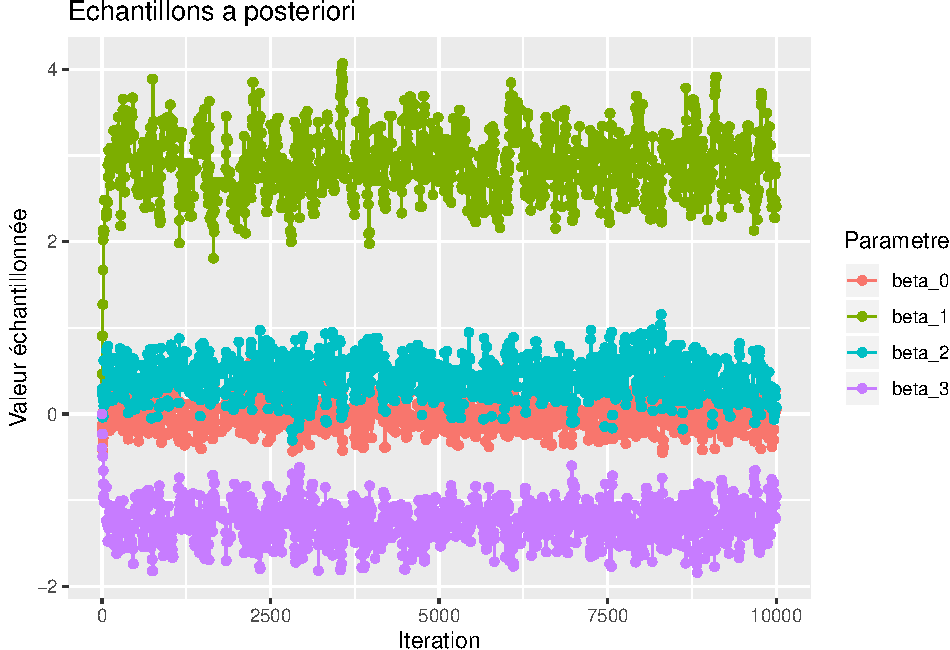
\includegraphics{correction_bayes_mcmc_files/figure-latex/plot_premier_mcmc-1.pdf}

\begin{Correction}
Il est \textbf{extrêmement important} de vérifier que le point de départ n'influe pas sur les valeurs échantillonnées (au moins au bout d'un certain temps).

Cela revient à s'assurer que, quelque soit le point de départ, on a bien atteint la loi stationnaire. Ici, on vérifie que pour la valeur de $\beta_1$, il n'y a pas d'influence du point de départ.
\end{Correction}

\begin{Shaded}
\begin{Highlighting}[]
\KeywordTok{set.seed}\NormalTok{(}\DecValTok{123}\NormalTok{)}
\NormalTok{mcmc_multiple_start <-}\StringTok{ }\KeywordTok{rerun}\NormalTok{(}\DecValTok{5}\NormalTok{,}
                             \KeywordTok{get_metropolis_sampling}\NormalTok{(}\KeywordTok{rnorm}\NormalTok{(}\DecValTok{4}\NormalTok{), }
                                                     \DataTypeTok{X =}\NormalTok{ design_matrix, }
                                                     \DataTypeTok{y =}\NormalTok{ y_vector, }
                                                     \DataTypeTok{n_step =} \FloatTok{1e3}\NormalTok{, }\DataTypeTok{sigma2 =} \FloatTok{0.1}\NormalTok{)) }\OperatorTok\StringTok{ }
\StringTok{  }\KeywordTok{bind_rows}\NormalTok{(}\DataTypeTok{.id =} \StringTok{"Replicate"}\NormalTok{)}
\KeywordTok{ggplot}\NormalTok{(mcmc_multiple_start) }\OperatorTok{+}
\StringTok{  }\KeywordTok{aes}\NormalTok{(}\DataTypeTok{x =}\NormalTok{ iteration, }\DataTypeTok{y =}\NormalTok{ beta_}\DecValTok{1}\NormalTok{, }\DataTypeTok{colour =}\NormalTok{ Replicate) }\OperatorTok{+}
\StringTok{  }\KeywordTok{geom_line}\NormalTok{() }\OperatorTok{+}
\StringTok{  }\KeywordTok{geom_point}\NormalTok{() }\OperatorTok{+}
\StringTok{  }\KeywordTok{labs}\NormalTok{(}\DataTypeTok{y =} \StringTok{"Valeur échantillonnée"}\NormalTok{, }\DataTypeTok{x =} \StringTok{"Iteration"}\NormalTok{, }
       \DataTypeTok{title =} \KeywordTok{expression}\NormalTok{(}\StringTok{"Echantillons de"}\OperatorTok{~}\NormalTok{beta[}\DecValTok{1}\NormalTok{]}\OperatorTok{~}\StringTok{"pour différents"}\OperatorTok{~}\NormalTok{sigma}\OperatorTok{^}\DecValTok{2}\NormalTok{),}
       \DataTypeTok{color =} \StringTok{"Pt de départ"}\NormalTok{)}
\end{Highlighting}
\end{Shaded}

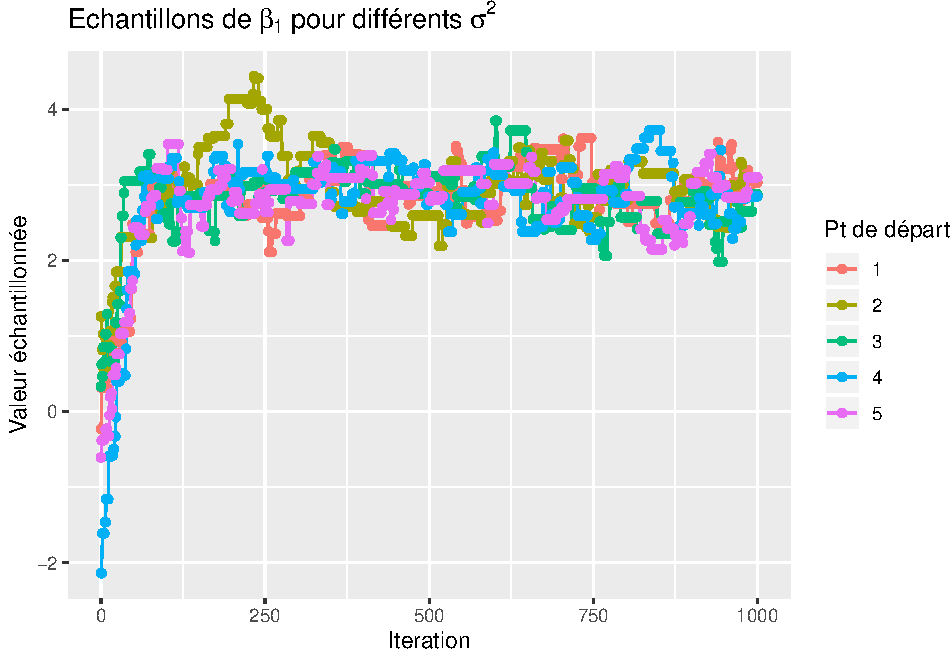
\includegraphics{correction_bayes_mcmc_files/figure-latex/mcmc_multiple_start-1.pdf}

\begin{Correction}
\textbf{Choix de $\sigma^2$} On peut regarder l'évolution de la chaîne selon la valeur de $\sigma^2$ choisie.
\end{Correction}

\begin{Shaded}
\begin{Highlighting}[]
\KeywordTok{set.seed}\NormalTok{(}\DecValTok{123}\NormalTok{)}
\NormalTok{mcmc_multiple_sigma <-}\StringTok{ }\KeywordTok{map_dfr}\NormalTok{(}\KeywordTok{c}\NormalTok{(}\FloatTok{1e-3}\NormalTok{, }\FloatTok{1e-2}\NormalTok{, }\FloatTok{1e-1}\NormalTok{, }\DecValTok{1}\NormalTok{),}
                               \ControlFlowTok{function}\NormalTok{(my_sigma)}
                                 \KeywordTok{get_metropolis_sampling}\NormalTok{(}\KeywordTok{rep}\NormalTok{(}\DecValTok{0}\NormalTok{, }\DecValTok{4}\NormalTok{), }
                                                         \DataTypeTok{X =}\NormalTok{ design_matrix, }
                                                         \DataTypeTok{y =}\NormalTok{ y_vector, }
                                                         \DataTypeTok{n_step =} \FloatTok{1e3}\NormalTok{, }
                                                         \DataTypeTok{sigma2 =}\NormalTok{ my_sigma))}
\KeywordTok{ggplot}\NormalTok{(mcmc_multiple_sigma) }\OperatorTok{+}
\StringTok{  }\KeywordTok{aes}\NormalTok{(}\DataTypeTok{x =}\NormalTok{ iteration, }\DataTypeTok{y =}\NormalTok{ beta_}\DecValTok{1}\NormalTok{, }\DataTypeTok{colour =} \KeywordTok{factor}\NormalTok{(sigma2)) }\OperatorTok{+}
\StringTok{  }\KeywordTok{geom_line}\NormalTok{() }\OperatorTok{+}
\StringTok{  }\KeywordTok{geom_point}\NormalTok{() }\OperatorTok{+}
\StringTok{  }\KeywordTok{labs}\NormalTok{(}\DataTypeTok{y =} \StringTok{"Valeur échantillonnée"}\NormalTok{, }\DataTypeTok{x =} \StringTok{"Iteration"}\NormalTok{, }
       \DataTypeTok{title =} \KeywordTok{expression}\NormalTok{(}\StringTok{"Echantillons de"}\OperatorTok{~}\NormalTok{beta[}\DecValTok{1}\NormalTok{]}\OperatorTok{~}\StringTok{"pour différents"}\OperatorTok{~}\NormalTok{sigma}\OperatorTok{^}\DecValTok{2}\NormalTok{),}
       \DataTypeTok{color =} \KeywordTok{expression}\NormalTok{(sigma}\OperatorTok{^}\DecValTok{2}\NormalTok{))}
\end{Highlighting}
\end{Shaded}

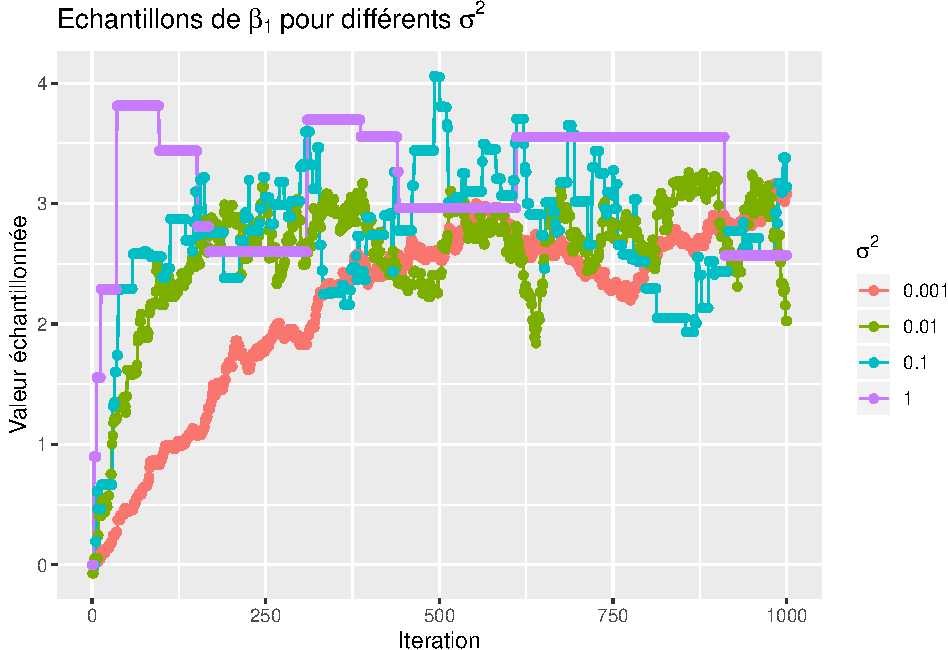
\includegraphics{correction_bayes_mcmc_files/figure-latex/mcmc_multiple_sigma-1.pdf}

\begin{Correction}
Pour les deux cas extrêmes, on voit deux comportements problématiques. 

Pour $\sigma^2 = 1$, on voit que la chaîne reste bloquée sur les mêmes valeurs la plupart du temps. ce qui implique en pratique que tout estimateur d'espérance selon la loi de $\sigma^2\vert \mathbf{y}, \mathbf{X}$ aura une très grande variance. 

Pour $\sigma^2 = 0.001$, on voit que la chaîne progresse lentement, cette chaîne présente donc une forte autocorrelation. Ceci implique également en pratique que tout estimateur d'espérance selon la loi de $\sigma^2\vert \mathbf{y}, \mathbf{X}$ aura une très grande variance.
Ici, $\sigma^2 = 0.01$ semble un bon compromis.
\end{Correction}

\begin{enumerate}
\def\labelenumi{\arabic{enumi}.}
\setcounter{enumi}{3}
\tightlist
\item
  Pour le \(\sigma^2\) choisi quelle est la probabilité d'acceptation
  empirique?
\end{enumerate}

\begin{Correction}
On obtient les taux d'acceptations suivants
\end{Correction}

\begin{Shaded}
\begin{Highlighting}[]
\NormalTok{mcmc_multiple_sigma }\OperatorTok\StringTok{ }
\StringTok{  }\KeywordTok{group_by}\NormalTok{(sigma2) }\OperatorTok\StringTok{ }
\StringTok{  }\KeywordTok{summarise}\NormalTok{(}\DataTypeTok{taux_acceptation =} \KeywordTok{mean}\NormalTok{(accepted, }\DataTypeTok{na.rm =} \OtherTok{TRUE}\NormalTok{)) }\OperatorTok\StringTok{ }
\StringTok{  }\NormalTok{knitr}\OperatorTok{::}\KeywordTok{kable}\NormalTok{(}\DataTypeTok{col.names =} \KeywordTok{c}\NormalTok{(}\StringTok{"$}\CharTok{\textbackslash{}\textbackslash{}}\StringTok{sigma^2$"}\NormalTok{, }\StringTok{"Taux d'acceptation"}\NormalTok{))}
\end{Highlighting}
\end{Shaded}

\begin{longtable}[]{@{}rr@{}}
\toprule
\(\sigma^2\) & Taux d'acceptation\tabularnewline
\midrule
\endhead
0.001 & 0.781\tabularnewline
0.010 & 0.515\tabularnewline
0.100 & 0.147\tabularnewline
1.000 & 0.013\tabularnewline
\bottomrule
\end{longtable}

\begin{Correction}
On peut regarder également l'autocorrélation de la chaîne (pour $\beta_1$, ici)
\end{Correction}

\begin{Shaded}
\begin{Highlighting}[]
\NormalTok{mcmc_multiple_sigma }\OperatorTok\StringTok{ }
\StringTok{  }\KeywordTok{group_by}\NormalTok{(sigma2) }\OperatorTok\StringTok{ }
\StringTok{  }\KeywordTok{summarise}\NormalTok{(}\DataTypeTok{autocorrel =} \KeywordTok{cor}\NormalTok{(beta_}\DecValTok{1}\NormalTok{[}\OperatorTok{-}\DecValTok{1}\NormalTok{], beta_}\DecValTok{1}\NormalTok{[}\OperatorTok{-}\KeywordTok{n}\NormalTok{()])) }\OperatorTok\StringTok{ }
\StringTok{  }\NormalTok{knitr}\OperatorTok{::}\KeywordTok{kable}\NormalTok{(}\DataTypeTok{col.names =} \KeywordTok{c}\NormalTok{(}\StringTok{"$}\CharTok{\textbackslash{}\textbackslash{}}\StringTok{sigma^2$"}\NormalTok{, }\StringTok{"Autocorrelation"}\NormalTok{))}
\end{Highlighting}
\end{Shaded}

\begin{longtable}[]{@{}rr@{}}
\toprule
\(\sigma^2\) & Autocorrelation\tabularnewline
\midrule
\endhead
0.001 & 0.9993751\tabularnewline
0.010 & 0.9917581\tabularnewline
0.100 & 0.9835038\tabularnewline
1.000 & 0.9864433\tabularnewline
\bottomrule
\end{longtable}

\begin{enumerate}
\def\labelenumi{\arabic{enumi}.}
\setcounter{enumi}{4}
\tightlist
\item
  Quelle est la valeur réalisée de l'estimateur Bayésien
  \(\mathbb{E}[\theta \vert \mathbf{Y}]\)?
\end{enumerate}

\begin{Correction}
On a désormais accès aux tirages de la chaîne de Markov qui a pour loi stationnaire notre loi cible. En pratique, pour estimer des espérances selon cette loi, on utilisera des méthodes de Monte Carlo standard, i.e., supposant que chaque tirage est i.i.d. de la loi voulue. 

Or cette hypothèse est violée ici pour deux raisons:

\begin{enumerate}
\item Les échantillons ne sont pas indépendants car ils sont issus d'une chaîne de Markov. Cependant, pour deux valeurs distantes de la chaîne, on peut penser que cette hypothèse d'indépendance sera valable.
\item Les échantillons ne sont pas tirés selon la loi cible. Asymptotiquement, on pourra le supposer, mais le point de départ n'est pas dans cette loi cible. On peut supposer cependant qu'au bout d'un certain temps, la chaîne a atteint la loi stationnaire.
\end{enumerate}

Afin de palier ces deux problèmes, on va sous échantillonné la chaîne de Markov selon deux principes, le \textit{thinning} et le \textit{burn-in}.

\begin{enumerate}
\item On choisit un écart temporel (le \textit{thin}) au delà duquel on suppose que toutes les valeurs de la chaîne sont indépendantes. En pratique, en gardera un point sur 10, un point sur 100, un point sur 1000,... selon l'autocorrelation initiale de la chaîne.
\item On choisit un pas de temps (le \textit{burn}) en deça duquel on jettera tous les échantillons, car on suppose que la chaîne n'a pas encore atteint sa loi stationnaire. De même, le choix de ce pas dépendra des données, et devra être justifié au moins graphiquement.
\end{enumerate}

Ici, on garde $\sigma^2 = 0.01$, on voit sur les graphes précédents qu'un \textit{burn-in} de 200 semble raisonnable (il faudrait vérifier sur les autres paramètres!). On gardera un point sur 100. Afin d'avoir un nombre surffisant de points pour l'approximation de l'espérance par méthode de Monte Carlo, on augmentera le nombre d'itérations.

On pourra vérifier ici que l'autocorrelation diminue en deça de 0.1 avec ces valeurs.

\end{Correction}

\begin{Shaded}
\begin{Highlighting}[]
\KeywordTok{set.seed}\NormalTok{(}\DecValTok{123}\NormalTok{)}
\NormalTok{my_mcmc_sample <-}\StringTok{ }\KeywordTok{get_metropolis_sampling}\NormalTok{(}\KeywordTok{rep}\NormalTok{(}\DecValTok{0}\NormalTok{, }\DecValTok{4}\NormalTok{), }\CommentTok{# On fait un metropolis}
                                          \DataTypeTok{X =}\NormalTok{ design_matrix, }
                                          \DataTypeTok{y =}\NormalTok{ y_vector, }
                                          \DataTypeTok{n_step =} \FloatTok{5e4}\NormalTok{, }\DataTypeTok{sigma2 =} \FloatTok{0.01}\NormalTok{) }\OperatorTok\StringTok{ }
\StringTok{  }\CommentTok{# Puis on ne garde qu'un sous ensemble des points}
\StringTok{  }\NormalTok{dplyr}\OperatorTok{::}\KeywordTok{filter}\NormalTok{(iteration }\OperatorTok{>=}\StringTok{ }\DecValTok{200}\NormalTok{, }\CommentTok{# Burn-in}
\NormalTok{                (iteration }\OperatorTok\StringTok{ }\DecValTok{100}\NormalTok{) }\OperatorTok{==}\StringTok{ }\DecValTok{0}\NormalTok{) }\CommentTok{# Thinning}
\end{Highlighting}
\end{Shaded}

\begin{Correction}
On pourra supposer que cet échantillon est i.i.d. de notre loi cible. On peut alors estimer l'espérance a posteriori de manière classique, en utilisant la moyenne empirique de cet échantillon.
\end{Correction}

\begin{longtable}[]{@{}lr@{}}
\toprule
Paramètre & Espérance a posteriori\tabularnewline
\midrule
\endhead
\(\beta_0\) & -0.023\tabularnewline
\(\beta_1\) & 2.906\tabularnewline
\(\beta_2\) & 0.412\tabularnewline
\(\beta_3\) & -1.265\tabularnewline
\bottomrule
\end{longtable}

\begin{enumerate}
\def\labelenumi{\arabic{enumi}.}
\setcounter{enumi}{5}
\tightlist
\item
  Donner un intervalle de crédibilité à 95\% pour chacun des paramètres.
\end{enumerate}

\begin{Correction}
De la même manière, un intervalle de crédiilité sera donné par les quantiles de niveaux correspondants.
\end{Correction}

\begin{Shaded}
\begin{Highlighting}[]
\NormalTok{my_mcmc_sample }\OperatorTok\StringTok{ }
\StringTok{  }\KeywordTok{select}\NormalTok{(beta_}\DecValTok{0}\NormalTok{, beta_}\DecValTok{1}\NormalTok{, beta_}\DecValTok{2}\NormalTok{, beta_}\DecValTok{3}\NormalTok{) }\OperatorTok\StringTok{ }
\StringTok{  }\KeywordTok{gather}\NormalTok{(}\DataTypeTok{key =} \StringTok{"Parametre"}\NormalTok{, }\DataTypeTok{value =} \StringTok{"Echantillon"}\NormalTok{, }\DataTypeTok{factor_key =} \OtherTok{TRUE}\NormalTok{) }\OperatorTok\StringTok{ }
\StringTok{  }\KeywordTok{group_by}\NormalTok{(Parametre) }\OperatorTok\StringTok{ }
\StringTok{  }\KeywordTok{summarise}\NormalTok{(}\DataTypeTok{IC_inf =} \KeywordTok{paste0}\NormalTok{(}\StringTok{"["}\NormalTok{, }
                            \KeywordTok{paste}\NormalTok{(}\KeywordTok{quantile}\NormalTok{(Echantillon, }\DataTypeTok{probs =} \KeywordTok{c}\NormalTok{(}\FloatTok{0.025}\NormalTok{,}\FloatTok{0.975}\NormalTok{)) }\OperatorTok\StringTok{ }
\StringTok{                                    }\KeywordTok{round}\NormalTok{(}\DecValTok{3}\NormalTok{),}
                                  \DataTypeTok{collapse =} \StringTok{", "}\NormalTok{),}
                            \StringTok{"]"}\NormalTok{)) }\OperatorTok\StringTok{ }
\StringTok{  }\KeywordTok{mutate}\NormalTok{(}\DataTypeTok{Parametre =} \KeywordTok{factor}\NormalTok{(Parametre, }
                            \DataTypeTok{labels =} \KeywordTok{paste0}\NormalTok{(}\StringTok{"$}\CharTok{\textbackslash{}\textbackslash{}}\StringTok{beta_"}\NormalTok{, }\DecValTok{0}\OperatorTok{:}\DecValTok{3}\NormalTok{,}\StringTok{"$"}\NormalTok{))) }\OperatorTok\StringTok{ }
\StringTok{  }\NormalTok{knitr}\OperatorTok{::}\KeywordTok{kable}\NormalTok{(}\DataTypeTok{col.names =} \KeywordTok{c}\NormalTok{(}\StringTok{"Paramètre"}\NormalTok{, }\StringTok{"Intervalle de crédibilité à 95 }\CharTok{\textbackslash{}\textbackslash{}}\StringTok{%"}\NormalTok{))}
\end{Highlighting}
\end{Shaded}

\begin{longtable}[]{@{}ll@{}}
\toprule
Paramètre & Intervalle de crédibilité à 95 \%\tabularnewline
\midrule
\endhead
\(\beta_0\) & {[}-0.317, 0.24{]}\tabularnewline
\(\beta_1\) & {[}2.324, 3.63{]}\tabularnewline
\(\beta_2\) & {[}-0.013, 0.836{]}\tabularnewline
\(\beta_3\) & {[}-1.709, -0.901{]}\tabularnewline
\bottomrule
\end{longtable}


\end{document}
